%%%%%%
%
% $Author: Abishek $
% $Date: 12.01.2025 $
% $Path: ML24-02-Gait-Pattern-Recognition\report\Contents\en$
% $Version: 1.0 $
%
%
% !TeX encoding = utf8
% !TeX root = Rename
% !TeX TXS-program:bibliography = txs:///bibtex
%
%%%%%%

	
	
	\section{Specific Sensor: Accelerometer (LSM9DS1)}
	
	An accelerometer is an electromechanical device used to measure acceleration forces. Such forces may be static, like the continuous force of gravity or, as is the case with many mobile devices, dynamic to sense movement or vibrations. The LSM9DS1 \ref{fig:lsm9ds1} is a sensor that combines three different tools: an accelerometer, a gyroscope, and a magnetometer. Among these, the accelerometer is used to measure how fast something is speeding up or slowing down in a straight line\cite{Alushi2024}. It does this by sensing motion along three directions:
	
\begin{figure}[h]
	\centering
	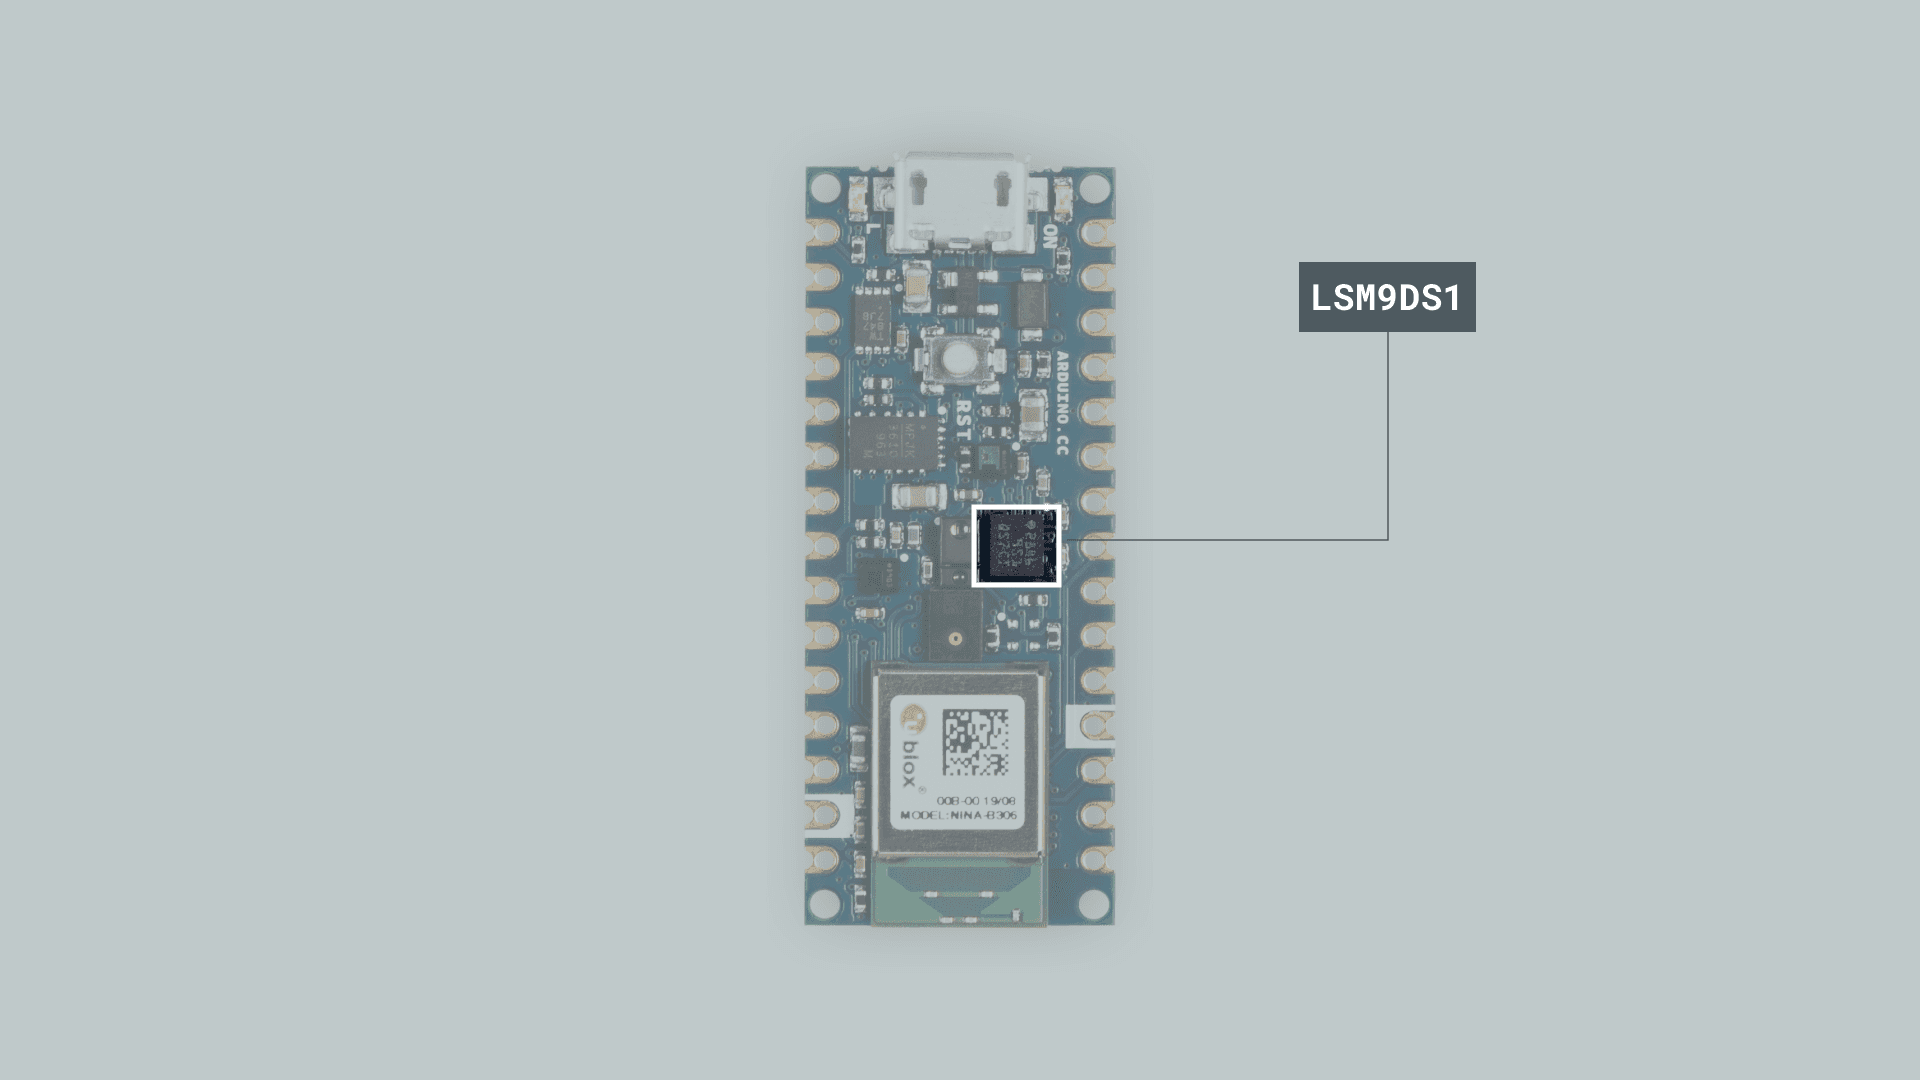
\includegraphics[width=0.7\textwidth]{Images/LSM9DS1}
	\caption{The LSM9DS1 sensor.\cite{Alushi2024}}
	\label{fig:lsm9ds1}
\end{figure}

	\begin{itemize}
		\item \textbf{X-axis:} Side-to-side motion.
		\item \textbf{Y-axis:} Forward and backward motion.
		\item \textbf{Z-axis:} Up and down motion (or gravity)\ref{fig:AxesRepresentation}\ref{fig:3axesAccelerometer}.
	\end{itemize}
	\begin{figure}[h]
	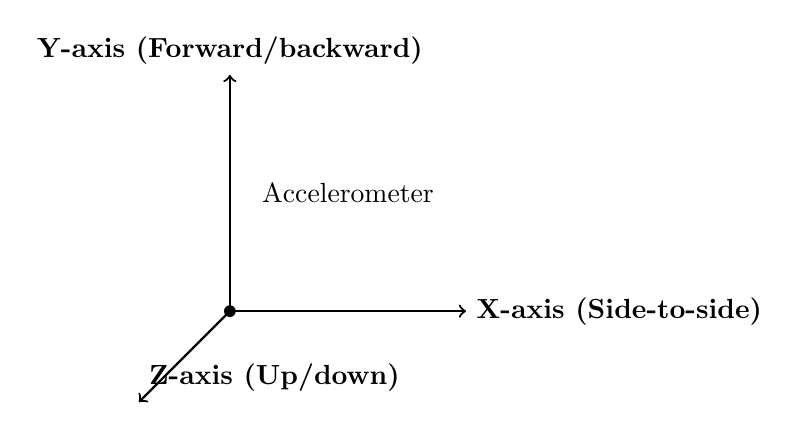
\begin{tikzpicture}[scale=1.5]
		\draw[->, thick] (0,0,0) -- (2,0,0) node[right] {\textbf{X-axis (Side-to-side)}};
		\draw[->, thick] (0,0,0) -- (0,2,0) node[above] {\textbf{Y-axis (Forward/backward)}};
		\draw[->, thick] (0,0,0) -- (0,0,2) node[above right] {\textbf{Z-axis (Up/down)}};
		\node at (0,0,0) [circle, fill, inner sep=1.5pt] {};
		\node at (1,1,0) {Accelerometer};
	\end{tikzpicture}
	\caption{Accelerometer Axes Representation}
	\label{fig:AxesRepresentation}
\end{figure}
	The accelerometer helps us understand how an object is moving or tilted. For example, if the sensor is lying flat on a table, it will detect gravity pulling down, showing about $1g$ (one unit of gravitational force) on the Z-axis, while the X and Y axes will stay close to $0g$. If you pick up the sensor and tilt it, the accelerometer will show different values depending on the tilt direction and angle.
	
	\begin{figure}[h]
		\centering
		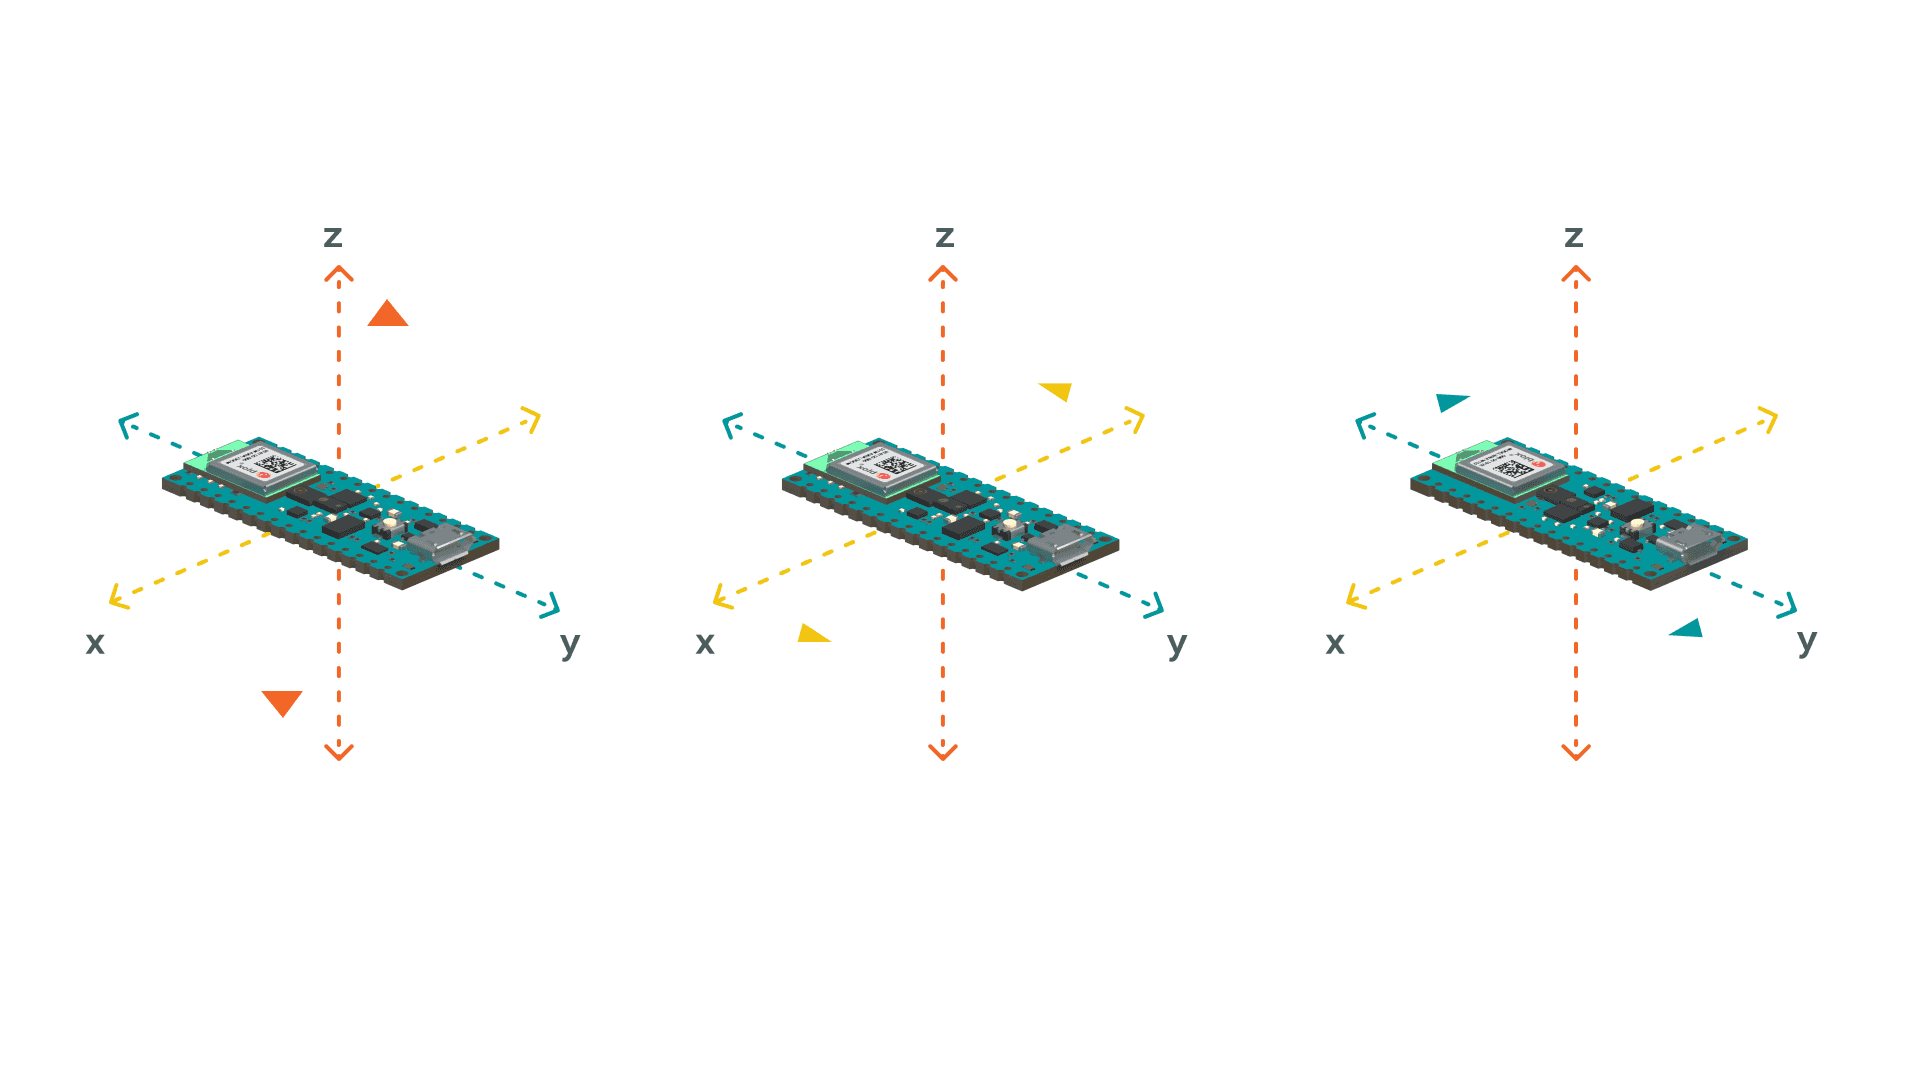
\includegraphics[width=0.7\textwidth]{Images/3axesAccelerometer}
		\caption{How the accelerometer works.\cite{Alushi2024}}
		\label{fig:3axesAccelerometer}
	\end{figure}
	
	The LSM9DS1 accelerometer is highly flexible and can work in many situations. It can measure slow, precise movements, like tilting a smartphone, or fast, high-impact events, like detecting a sudden fall or collision. This is why it’s used in devices like fitness trackers, drones, smartphones, and gaming controllers.\cite{Yang:2010}
	
	The accelerometer works using \textbf{MEMS (Micro-Electro-Mechanical Systems)} technology, which involves tiny mechanical parts inside the sensor. When the sensor moves, these parts shift slightly, creating electrical signals. The sensor converts these signals into data that tells you how the object is moving or tilting.\cite{Khoshnoud:2012}
	
	This sensor is small, energy-efficient, and easy to connect to microcontrollers like the Arduino Nano 33 BLE Sense, making it perfect for portable, battery-powered devices. It can even measure tiny changes in motion, making it useful for delicate tasks like detecting small vibrations in machinery or tracking a slight tilt in a device.\cite{Mutlu:2021}
	
	However, like all sensors, the accelerometer isn’t perfect. It can sometimes pick up noise, which means the data might not always be 100\% accurate. Temperature changes or long-term use can also cause small errors, so it’s important to calibrate the sensor regularly to keep it accurate.
	
	Despite these challenges, the LSM9DS1 accelerometer is a powerful and reliable tool for measuring motion and tilt. Its ability to work in many different environments makes it an essential part of modern technology, from fitness and healthcare to gaming and robotics\cite{Nistler:2011}.
	
	
	\section{Specification for LSM9DS1 Accelerometer}	
	
	The accelerometer in the LSM9DS1 is a high-performance 3-axis sensor designed to measure linear acceleration along the X, Y, and Z axes. Below are the detailed specifications:
	
	
	\begin{table}[h!]
		\centering
		\begin{tabular}{|l|l|}
			\hline
			\textbf{Specification}         & \textbf{Details}                         \\ \hline
			\textbf{Measurement Ranges}    & ±2g, ±4g, ±8g, ±16g (configurable)       \\ \hline
			\textbf{Resolution}            & 16-bit digital output                    \\ \hline
			\textbf{Sensitivity}           & Detects small changes in acceleration:   \\
			& ±2g: 0.061 mg/LSB                        \\ \hline
			\textbf{Output Data Rate (ODR)}& Configurable from 10 Hz to 952 Hz         \\ \hline
			\textbf{Power Consumption}     & Normal: 600 µA                           \\
			& Low-Power: 240 µA                        \\
			& Standby: 1 µA                            \\ \hline
			\textbf{Operating Voltage}     & 1.9 V to 3.6 V                           \\ \hline
			\textbf{Shock Resistance}      & Handles up to 10,000g for short impacts  \\ \hline
			\textbf{Communication Interfaces} & I²C (up to 400 kHz), SPI (up to 10 MHz) \\ \hline
			\textbf{Temperature Range}     & -40°C to +85°C                           \\ \hline
		\end{tabular}
		\caption{Specifications of the LSM9DS1 Accelerometer.\cite{STM:2015}}
	\end{table}
	
	\subsection*{Explanations}
	
	\textbf{Measurement Ranges:} The accelerometer measures acceleration in configurable ranges. Smaller ranges like ±2g are suitable for precise motion detection, while larger ranges like ±16g are ideal for high-impact events.
	
	\textbf{Resolution:} The sensor provides 16-bit resolution, capturing detailed changes in motion for accurate measurements.
	
	\textbf{Sensitivity:} Sensitivity determines the smallest motion the sensor can detect. For example, in the ±2g range, it detects changes as small as 0.061 mg (0.000061 g).
	
	\textbf{Output Data Rate (ODR):} The ODR specifies how often the sensor updates its data. Low rates like 10 Hz are suitable for slow motions, while high rates like 952 Hz are ideal for fast, real-time tracking.
	
	\textbf{Power Consumption:} The accelerometer operates in three modes:
	\begin{itemize}
		\item \textbf{Normal Mode:} Uses 600 µA for active motion sensing.
		\item \textbf{Low-Power Mode:} Uses 240 µA for energy-efficient applications.
		\item \textbf{Standby Mode:} Uses just 1 µA when idle.
	\end{itemize}
	
	\textbf{Operating Voltage:} The sensor operates between 1.9 V and 3.6 V, making it compatible with various power sources.
	
	\textbf{Shock Resistance:} It is highly durable, handling short impacts up to 10,000g, making it ideal for high-stress applications.
	
	\textbf{Communication Interfaces:} The accelerometer communicates with microcontrollers using:
	\begin{itemize}
		\item \textbf{I²C:} A slower, simple protocol for most applications.
		\item \textbf{SPI:} A faster option for high-speed, real-time tasks.
	\end{itemize}
	
	\textbf{Temperature Range:} Operates reliably in extreme temperatures from -40°C to +85°C, suitable for a wide range of environments.\cite{STM:2015}
	
\section{Library for LSM9DS1 Accelerometer}

The \textbf{Arduino\_LSM9DS1} library is designed to interface with the LSM9DS1 accelerometer on the Arduino Nano 33 BLE Sense. It simplifies tasks like initializing the sensor, configuring its settings, and reading acceleration data. Key functions provided by the library include \texttt{IMU.begin()} for sensor initialization, \texttt{IMU.accelerationAvailable()} to check for new data, and \texttt{IMU.readAcceleration(x, y, z)} to retrieve acceleration values along the X, Y, and Z axes. By handling low-level communication protocols internally, the library enables developers to focus on building applications without dealing with complex configurations.

\subsection*{Installing the Library}

\begin{enumerate}
	\item \textbf{Open Arduino IDE}:  
	Launch the Arduino Integrated Development Environment (IDE) on your computer.
	
	\item \textbf{Go to the Library Manager}:  
	In the top menu, click on \texttt{Sketch} $\rightarrow$ \texttt{Include Library} $\rightarrow$ \texttt{Manage Libraries}.
	
	\item \textbf{Search for the Library}:  
	In the Library Manager window, type \texttt{Arduino\_LSM9DS1} in the search bar.
	
	\item \textbf{Install the Library}:  
	When the library appears in the search results, click on the \texttt{Install} button next to it.
	
	\item \textbf{Wait for Installation to Complete}:  
	The Arduino IDE will automatically download and install the library. Once it's done, you can close the Library Manager.
	
	\item \textbf{Verify Installation}:  
	To check if the library is installed successfully, go to \texttt{Sketch} $\rightarrow$ \texttt{Include Library} $\rightarrow$ \texttt{Arduino\_LSM9DS1}. It should appear in the list of available libraries.
\end{enumerate}

After completing these steps, the \texttt{Arduino\_LSM9DS1} library will be ready for use in your Arduino projects to access and control the accelerometer sensor on the Arduino Nano 33 BLE Sense\cite{Alushi2024}



\section{Calibration of LSM9DS1 Accelerometer}

Calibration is the process of adjusting a sensor’s output to correct for inaccuracies, ensuring it provides accurate and reliable data across its specified range. This process is essential to account for errors that may arise due to manufacturing variances, environmental factors, or the sensor's natural drift over time. Calibration helps eliminate these systematic errors, often involving comparisons to known reference values or mathematical adjustments\cite{Oh:2017}.

Calibration is crucial for ensuring the LSM9DS1 accelerometer provides accurate and consistent data. Factors like temperature changes, mechanical impacts, or manufacturing variations can introduce small errors, known as offsets, in the sensor's readings.\cite{STM:2015} These offsets can cause deviations from expected values, such as when the sensor is stationary and flat, where the X and Y axes should read 0g, and the Z-axis should read 1g due to gravity. Calibration involves determining these offsets and adjusting the sensor's raw output accordingly, improving the precision of acceleration measurements.\cite{fraden:2016}

To calibrate the accelerometer, the sensor is placed on a stable, flat surface, and the raw acceleration readings are recorded for each axis. The differences between the measured and expected values (offsets) are calculated and applied programmatically to correct future readings. Calibration enhances the sensor's accuracy and reliability, especially in applications like motion tracking and tilt sensing. It is recommended to perform recalibration periodically or after significant environmental or physical changes to maintain consistent performance.

The following code demonstrates how to calibrate the LSM9DS1 accelerometer using the Arduino\_LSM9DS1 library, which provides functions for reading sensor data and applying calibration offsets\cite{arduinolsm9ds1}.

\begin{lstlisting}[language=C++, caption=Calibration Code for LSM9DS1 Accelerometer]
	
	#include <Arduino_LSM9DS1.h>  // Include the library
	
	// Calibration offsets (calculated during calibration process)
	float offsetX = -0.05;  // Example X-axis offset
	float offsetY = 0.02;   // Example Y-axis offset
	float offsetZ = 0.05;   // Example Z-axis offset
	
	void setup() {
		Serial.begin(9600);        // Start Serial Monitor
		while (!Serial);           // Wait for connection
		
		if (!IMU.begin()) {        // Initialize accelerometer
			Serial.println("Failed to initialize IMU!");
			while (1);               // Halt if initialization fails
		}
		Serial.println("IMU initialized. Calibration offsets applied.");
	}
	
	void loop() {
		float x, y, z;
		
		if (IMU.accelerationAvailable()) {          // Check if data is available
			IMU.readAcceleration(x, y, z);            // Read raw acceleration data
			
			// Apply calibration offsets
			x += offsetX;
			y += offsetY;
			z += offsetZ;
			
			Serial.print("Calibrated Acceleration -> X: ");
			Serial.print(x);
			Serial.print(" g, Y: ");
			Serial.print(y);
			Serial.print(" g, Z: ");
			Serial.println(z);
		}
		delay(100);                                 // Wait before reading again
	}
\end{lstlisting}

	This code demonstrates how to calibrate the LSM9DS1 accelerometer by applying predefined offsets to raw acceleration data. The offsets (offsetX, offsetY, offsetZ) are calculated by measuring the difference between the expected values (e.g., 0g for X and Y, 1g for Z) and the raw sensor readings when the device is flat and stationary. These offsets are then added to the raw acceleration readings in real time, ensuring corrected and accurate values are displayed on the Serial Monitor. This method provides a simple and effective way to compensate for sensor errors and improve data reliability.\cite{arduinolsm9ds1}
	
	\section{Simple Code to Read Acceleration Data}
	
	\begin{lstlisting}[language=C++, caption=Basic Code for LSM9DS1 Accelerometer\cite{arduinolsm9ds1}]
		
		
		#include <Arduino_LSM9DS1.h>  // Include the library
		
		void setup() {
			Serial.begin(9600);        // Start the Serial Monitor
			while (!Serial);           // Wait for the Serial Monitor to connect
			
			if (!IMU.begin()) {        // Initialize the accelerometer
				Serial.println("Failed to initialize IMU!");
				while (1);               // Halt the program if initialization fails
			}
			Serial.println("IMU initialized.");
		}
		
		void loop() {
			float x, y, z;
			
			if (IMU.accelerationAvailable()) {          // Check if new data is ready
				IMU.readAcceleration(x, y, z);            // Read acceleration data
				Serial.print("X: ");
				Serial.print(x);                          // Print X-axis data
				Serial.print(" g, Y: ");
				Serial.print(y);                          // Print Y-axis data
				Serial.print(" g, Z: ");
				Serial.println(z);                        // Print Z-axis data
			}
			delay(100);                                 // Wait before reading again
		}
		
	\end{lstlisting}
	
	
	The code initializes the LSM9DS1 accelerometer on the Arduino Nano 33 BLE Sense using the \texttt{IMU.begin()} function, ensuring the sensor is ready to collect data. In the main loop, it checks for new acceleration data with \texttt{IMU.accelerationAvailable()}, and if available, retrieves the X, Y, and Z axis values using \texttt{IMU.readAcceleration(x, y, z)}. These values represent motion or tilt in three directions and are printed to the Serial Monitor in units of gravitational force (\texttt{g}). The program updates the readings every 100 milliseconds, allowing continuous monitoring of acceleration.
	
	\section{Simple Application}
	
	A common application of the LSM9DS1 accelerometer is tilt detection, where the accelerometer detects the angle at which an object is tilted. This is used in various devices, such as smartphones for screen orientation or drones for flight stabilization.
	

\begin{lstlisting}[language=C++, caption=Code for Tilt Detection and Angle Calculation\cite{Alushi2024}]
	
#include <Arduino_LSM9DS1.h>

float x, y, z;
int degreesX = 0;
int degreesY = 0;

void setup() {
	Serial.begin(9600);
	while (!Serial);
	Serial.println("Started");
	
	if (!IMU.begin()) {
		Serial.println("Failed to initialize IMU!");
		while (1);
	}
	
	Serial.print("Accelerometer sample rate = ");
	Serial.print(IMU.accelerationSampleRate());
	Serial.println("Hz");
}

void loop() {
	
	if (IMU.accelerationAvailable()) {
		IMU.readAcceleration(x, y, z);
		
	}
	
	if (x > 0.1) {
		x = 100 * x;
		degreesX = map(x, 0, 97, 0, 90);
		Serial.print("Tilting up ");
		Serial.print(degreesX);
		Serial.println(" degrees");
	}
	if (x < -0.1) {
		x = 100 * x;
		degreesX = map(x, 0, -100, 0, 90);
		Serial.print("Tilting down ");
		Serial.print(degreesX);
		Serial.println(" degrees");
	}
	if (y > 0.1) {
		y = 100 * y;
		degreesY = map(y, 0, 97, 0, 90);
		Serial.print("Tilting left ");
		Serial.print(degreesY);
		Serial.println(" degrees");
	}
	if (y < -0.1) {
		y = 100 * y;
		degreesY = map(y, 0, -100, 0, 90);
		Serial.print("Tilting right ");
		Serial.print(degreesY);
		Serial.println(" degrees");
	}
	delay(1000);
}
	\end{lstlisting}
	
	This code uses the LSM9DS1 accelerometer on the Arduino Nano 33 BLE Sense to detect tilt and calculate the angle in degrees along the X and Y axes. The program initializes the sensor with IMU.begin() and reads acceleration values using IMU.readAcceleration(x, y, z). When the acceleration on the X or Y axis exceeds a small threshold (±0.1g), the map() function converts the acceleration values into tilt angles ranging from 0° to 90°. Depending on the sign and magnitude of the acceleration, the program identifies the tilt direction (up, down, left, or right) and prints both the direction and angle to the Serial Monitor every second, providing real-time orientation feedback\cite{Alushi2024}.
	
	\section{Testing the Accelerometer}
	
	To ensure accurate readings from the board, hold the Arduino Nano 33 BLE Sense in your hand with the USB port facing you and the board pointing away from you. The board should be positioned flat, as shown in the image below\ref{fig:Interacting with the X and Y axes}. This setup helps you interact with the X and Y axes effectively while testing.
	
	\begin{figure}[h]
		\centering
		
\includegraphics[width=0.7\textwidth]{Images/nano33BS_02_illustration}
		\caption{Interacting with the X and Y axes.\cite{Alushi2024}}
		\label{fig:Interacting with the X and Y axes}
	\end{figure}
	
	\subsection{Running the Test}
	After uploading the sketch to the board, open the Serial Monitor from the Arduino IDE's menu to view the results. By tilting the board in different directions—upwards, downwards, left, or right—you can observe the readings in the Serial Monitor. The tilt direction and corresponding angles are displayed in real-time. For example, tilting the board upwards increases the X-axis values, while tilting to the left or right changes the Y-axis values.\cite{Alushi2024}
	Below image \ref{fig:Printing tilt} is a screenshot showing the tilt condition being displayed in the Serial Monitor:
		\begin{figure}[h]
		\centering
		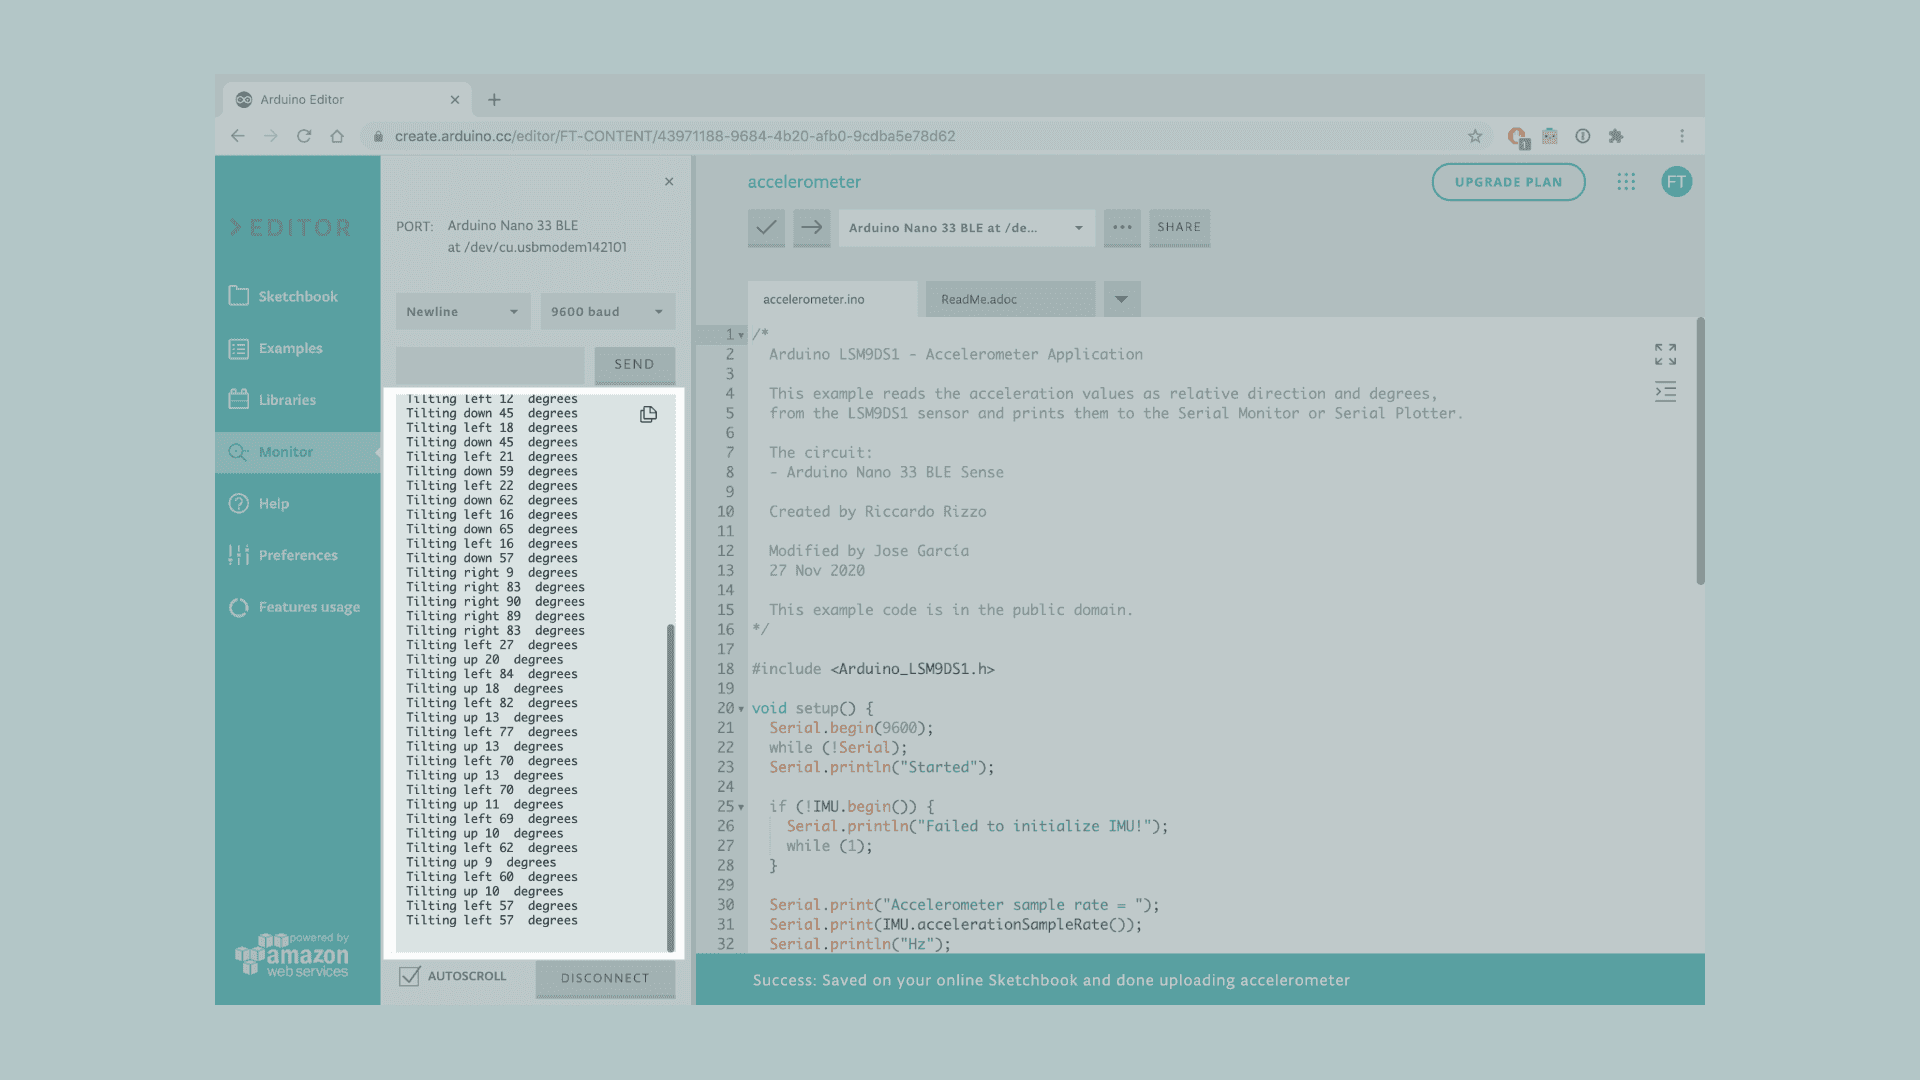
\includegraphics[width=0.7\textwidth]{Images/nano33BS_02_printing_values}
		\caption{Printing out the "tilt condition" of the board\cite{Alushi2024}}
		\label{fig:Printing tilt}
	\end{figure}
	